\documentclass[tikz]{standalone}
% \usetikzlibrary{intersections}
\input{../standalonepreamble.tex}

\begin{document}
\tikzset{help lines/.style=very thin}
\tikzset{Karl's grid/.style={help lines,color=blue!50}}

\begin{tikzpicture}[scale=1.5,>=Stealth,every node/.style={scale=0.5}]
%  \clip (-2,-0.2) rectangle (2,0.8);
  \draw[step=0.5cm,gray,very thin] (-1.4,-1.4) grid (1.4,1.4);
  \draw[->] (-1.5,0) -- (1.5,0) coordinate (x axis);
  \draw[->] (0,-1.5) -- (0,1.5) coordinate (y axis);
  \draw (0,0) circle [radius=1cm];
  \filldraw[fill=green!20!white, draw=green!50!black] (0,0) -- (3mm,0mm)
    arc [start angle=0, end angle=30, radius=3mm] -- cycle;
  \draw (15:2mm) node[color=green!50!black] {$\alpha$};
%   \shadedraw[left color=gray, right color=green, draw=green!50!black] (0,0) --
%   (3mm,0mm) arc [start angle=0, end angle=30, radius=3mm] -- cycle;
  \draw[red, very thick] (30:1cm) -- node [left=1pt,fill=white] {$\sin \alpha$}
        (30:1cm |- x axis);
  \draw[blue, very thick] (30:1cm |- x axis) -- node[below=2pt,fill=white] {$
        \cos \alpha$} (0,0);

  \path [name path=upward line] (1,0) -- (1,1);
  \path [name path=sloped line] (0,0) -- (30:1.5cm);
  \draw [name intersections={of=upward line and sloped line, by=t}][very thick,
          orange] (1,0) -- node [right=1pt, fill=white]{$\displaystyle \tan
          \alpha \color{black}=\frac{{\color{red}\sin \alpha}}{{\color{blue}\cos
          \alpha}}$} (t);

  \draw (0,0) -- (t);

  \foreach \x/\xtext in {-1, -0.5/-\frac{1}{2}, 1}
  \draw (\x cm,1pt) -- (\x cm, -1pt) node[anchor=north, fill=white] {$\xtext$};
  \foreach \y/\ytext in {-1,-0.5/-\frac{1}{2},0.5/\frac{1}{2},1}
  \draw (1pt,\y cm) -- (-1pt,\y cm) node[anchor=east, fill=white] {$\ytext$};
\end{tikzpicture}

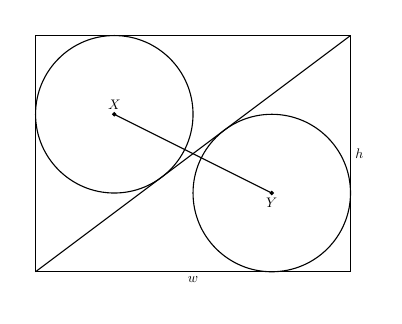
\begin{tikzpicture}[every node/.style={scale=0.5}]
  \clip (-0.1,-0.3) rectangle (4.3,3.1);
  \draw[thin] (0,0) rectangle (4,3);
  \draw (0,0) -- (4,3);
  \draw (1.0, 2.0) circle [radius=1cm];
  \draw (3.0, 1.0) circle [radius=1cm];
  \draw (1.0, 2.0) -- (3.0, 1.0);
  \filldraw (1.0, 2.0) circle [radius=0.2mm];
  \filldraw (3.0, 1.0) circle [radius=0.2mm];
  \draw (1.0,2.0) node[above] {$X$};
  \draw (3.0,1.0) node[below] {$Y$};
  \draw (2.0,0.0) node[below] {$w$};
  \draw (4.0,1.5) node[right] {$h$};
\end{tikzpicture}

\begin{tikzpicture}[scale=1]
\draw (.1,1.6) .. controls (.6,1.6) and (1.5,1) .. (2,1);
\begin{scope}
  \clip (1,0) rectangle (2,2);
  \draw (.1,1) .. controls (.6,1) and (1.5,.4) .. (2,.4);
\end{scope}
\draw[dashed] (1,0) -- (1,2);
\end{tikzpicture}

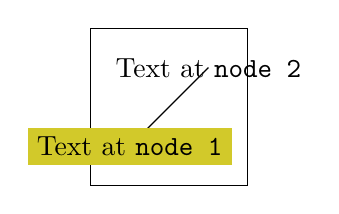
\begin{tikzpicture}
  \draw (0,0) rectangle (2,2);
  \draw (0.5,0.5) node [fill=yellow!80!black]
                       {Text at \verb!node 1!}
     -- (1.5,1.5) node {Text at \verb!node 2!};
\end{tikzpicture}

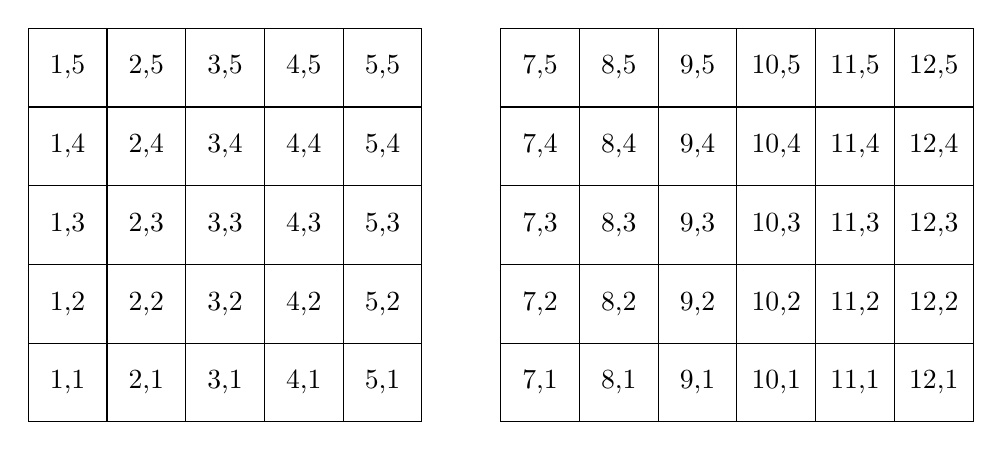
\begin{tikzpicture}[scale=1]
  \foreach \x in {1,2,...,5,7,8,...,12}
    \foreach \y in {1,...,5}
    {
      \draw (\x,\y) +(-0.5,-0.5) rectangle ++(0.5,0.5);
      \draw (\x,\y) node{\x,\y};
    }
\end{tikzpicture}

\end{document}
